\documentclass{article}

% NeurIPS 2025 style
\usepackage[preprint]{neurips_2025}

\usepackage[utf8]{inputenc}
\usepackage[T1]{fontenc}
\usepackage{hyperref}
\usepackage{url}
\usepackage{booktabs}
\usepackage{amsfonts}
\usepackage{amsmath}
\usepackage{amssymb}
\usepackage{nicefrac}
\usepackage{microtype}
\usepackage{xcolor}
\usepackage{graphicx}
\usepackage{listings}
\usepackage{algorithm}
\usepackage{algorithmic}
\usepackage{multirow}
\usepackage{subcaption}
\usepackage{tikz}
\usepackage{mdframed}
\usetikzlibrary{shapes,arrows,positioning,fit,backgrounds,calc}

\definecolor{codegray}{rgb}{0.5,0.5,0.5}
\definecolor{codepurple}{rgb}{0.58,0,0.82}
\definecolor{codeblue}{rgb}{0.0,0.0,0.8}
\definecolor{codegreen}{rgb}{0.0,0.5,0.0}
\definecolor{backcolour}{rgb}{0.97,0.97,0.97}

\lstdefinestyle{tscode}{
  backgroundcolor=\color{backcolour},
  commentstyle=\color{codegreen}\itshape,
  keywordstyle=\color{codeblue}\bfseries,
  stringstyle=\color{codepurple},
  basicstyle=\ttfamily\scriptsize,
  breakatwhitespace=false,
  breaklines=true,
  captionpos=b,
  keepspaces=true,
  numbers=left,
  numberstyle=\tiny\color{codegray},
  numbersep=5pt,
  showspaces=false,
  showstringspaces=false,
  showtabs=false,
  tabsize=2,
  frame=single,
  framesep=2pt,
  xleftmargin=8pt,
}

\lstset{style=tscode}

\newcommand{\file}[1]{\texttt{\small #1}}
\newcommand{\code}[1]{\texttt{#1}}
\newcommand{\insight}[1]{%
  \begin{mdframed}[backgroundcolor=blue!5, linecolor=blue!30, linewidth=0.5pt,
    topline=true, bottomline=true, leftline=true, rightline=true,
    innertopmargin=4pt, innerbottommargin=4pt]
  \small\textbf{Insight:} #1
  \end{mdframed}
}

% ─────────────────────────────────────────────────────────────
\title{%
  \textbf{Inside Claude Code: Architecture, Orchestration,}\\
  \textbf{and Governance of a Production LLM Coding Agent}
}

\author{%
  Anonymous Authors\\
  \textit{Under Review --- NeurIPS 2025}
}
% ─────────────────────────────────────────────────────────────

\begin{document}
\maketitle

% ─────────────────────────────────────────────────────────────
\begin{abstract}
% ─────────────────────────────────────────────────────────────
We present a systematic technical analysis of Claude Code v2.1.88, Anthropic's production command-line coding agent, based on its 1,884-file TypeScript source corpus ($\approx$163\,K lines of code). While prior agent frameworks (ReAct, LangChain, AutoGen) have established principled interaction patterns, the engineering realities of a production agent remain largely unstudied. Our analysis reveals five architectural contributions that go beyond prior academic treatments: \textbf{(1) a streaming, API-turn-grained agentic loop} with typed state-machine transitions and multi-level error recovery; \textbf{(2) tool-semantic concurrency}---a per-input, declarative concurrency model with tool-aware sibling-abort error propagation; \textbf{(3) three-tier context management} combining proactive session-memory extraction, auto-compaction with a circuit breaker, and non-destructive context folding; \textbf{(4) an AST-level, five-layer permission pipeline} integrating syntactic analysis, ML classification, and persistent rule learning; and \textbf{(5) a remote governance infrastructure} including hourly remote-settings polling, feature-flag killswitches, and a dual telemetry pipeline with no user-facing opt-out. We extract six design principles with broad applicability to future agentic systems and identify four open research problems motivated by the engineering choices observed.
\end{abstract}

% ─────────────────────────────────────────────────────────────
\section{Introduction}
% ─────────────────────────────────────────────────────────────

The ReAct framework~\cite{yao2022react} popularized the \textsc{Thought--Action--Observation} loop as a foundation for LLM agents, and subsequent works~\cite{shinn2023reflexion,wei2022chain,schick2023toolformer} have expanded our theoretical understanding of agent reasoning. Yet the path from a research prototype to a reliable production system involves a different class of challenges: How does one handle context overflow mid-task without losing the user's original intent? How does one safely orchestrate dozens of concurrent tool calls while preserving API-level ordering semantics? How does one give an agent meaningful autonomy while ensuring destructive actions are always gated on human approval?

Claude Code~\cite{anthropic2024claudecode}, Anthropic's CLI-based coding agent, provides a rare opportunity to study these questions through the lens of a mature production system. Its v2.1.88 npm package, comprising 1,884 TypeScript and TSX files across 11 subsystems, exposes concrete engineering decisions made to address each of these challenges at scale.

This paper makes four contributions:
\begin{enumerate}
  \item A systematic architectural analysis of a production LLM agent based on actual source code, covering five major subsystems with concrete algorithmic and data-structure detail.
  \item Identification of three novel engineering patterns---\emph{tool-semantic sibling abort}, \emph{AST-level permission evaluation}, and \emph{non-destructive context folding}---that have no direct counterpart in the academic literature.
  \item Extraction of six design principles and four open problems motivated by the gap between current research agent frameworks and production engineering requirements.
  \item A comparative analysis between the TypeScript production system and its Python clean-room reimplementation (\emph{claw-code}~\cite{clawcode2026}), illuminating which design decisions are essential versus incidental.
\end{enumerate}

% ─────────────────────────────────────────────────────────────
\section{Background}
% ─────────────────────────────────────────────────────────────

\subsection{LLM Agent Frameworks}

Early LLM agent systems used fixed reasoning templates: ReAct~\cite{yao2022react} interleaves chain-of-thought reasoning with tool invocations; Reflexion~\cite{shinn2023reflexion} adds a verbal self-evaluation loop; Plan-and-Solve~\cite{wang2023plan} separates planning from execution. Tool-use capability was acquired either by fine-tuning (Toolformer~\cite{schick2023toolformer}) or by prompting (ReAct). Coding-specific agents---SWE-agent~\cite{yang2024sweagent}, OpenHands~\cite{wang2024openhands}, Devin~\cite{cognition2024devin}---applied these ideas to software engineering benchmarks, but their system-level implementation details are not publicly disclosed.

\subsection{Multi-Agent Orchestration}

AutoGen~\cite{wu2023autogen} proposes conversable agents with code execution; MetaGPT~\cite{hong2023metagpt} assigns specialized roles to different model instances. Park et al.~\cite{park2023generative} demonstrate emergent social behavior in agent communities. Claude Code's Coordinator/Worker pattern is a principled production instance of hierarchical orchestration with explicit isolation guarantees not present in these frameworks.

\subsection{Context Management}

The ``lost-in-the-middle'' effect~\cite{liu2023lost} motivates context management strategies. RAG~\cite{lewis2020retrieval} addresses knowledge retrieval but not conversational history. Summarization-based compression~\cite{zhang2024survey} is the standard approach. Claude Code's three-tier strategy introduces \emph{agent-authored} session memory and circuit-breaker recovery, which have not been previously studied.

% ─────────────────────────────────────────────────────────────
\section{System Overview}
% ─────────────────────────────────────────────────────────────

\subsection{Codebase Scale and Organization}

\begin{table}[t]
\centering
\caption{Claude Code v2.1.88 subsystem summary. File counts exclude \texttt{vendor/} and \texttt{stubs/}.}
\label{tab:subsystems}
\small
\begin{tabular}{llrl}
\toprule
\textbf{Subsystem} & \textbf{Directory} & \textbf{\#Files} & \textbf{Largest file (KB)} \\
\midrule
Core agent loop   & \file{src/} (root)         & 27  & \file{query.ts} (785) \\
Tool impls.       & \file{src/tools/}          & 44 dirs & \file{BashTool/index.ts} (72) \\
Services          & \file{src/services/}       & 22 dirs & \file{StreamingToolExecutor.ts} (28) \\
Slash commands    & \file{src/commands/}       & 87  & --- \\
Terminal UI       & \file{src/components/}     & 33 dirs & --- \\
Utilities         & \file{src/utils/}          & 30+ & \file{bash/ast.ts} (64) \\
Bridge            & \file{src/bridge/}         & 6   & --- \\
Coordinator       & \file{src/coordinator/}    & 4   & --- \\
Analytics         & \file{src/services/analytics/} & 12 & --- \\
Memory            & \file{src/memdir/}         & 5   & --- \\
Tasks             & \file{src/tasks/}          & 5   & --- \\
\bottomrule
\end{tabular}
\end{table}

Table~\ref{tab:subsystems} summarizes the 11 top-level subsystems. The runtime is Bun, compiling the entire codebase into a single Node.js $\geq$18 bundle via esbuild. The terminal UI uses React rendered through Ink~\cite{ink2023}. The agent exposes four execution modes: interactive CLI (REPL), headless/SDK (programmatic), remote (SSH/Teleport), and Desktop Bridge. Our analysis focuses on the CLI and SDK modes.

% ─────────────────────────────────────────────────────────────
\section{The Streaming Agentic Loop}
\label{sec:loop}
% ─────────────────────────────────────────────────────────────

\subsection{API-Turn Granularity}

A key design decision distinguishes Claude Code from simpler agent implementations: the inner execution loop iterates over \emph{API turns}, not \emph{user turns}. Each API turn corresponds to one streaming request to the Claude API. When the response contains tool calls, they are executed and appended as \code{tool\_result} blocks, immediately triggering the next API turn---without waiting for user input. A single user message may generate dozens of API turns as the agent performs multi-step file edits, searches, and shell commands.

This decoupling is implemented as a typed state machine in \file{src/query.ts}:

\begin{lstlisting}[language=TypeScript, caption={Core state machine type in \texttt{query.ts}.}, label={lst:state}]
type QueryState = {
  messages:               Message[]
  toolUseContext:         ToolUseContext
  maxOutputTokensRecovery: number      // circuit-breaker counter
  hasAttemptedReactiveCompact: boolean // idempotency guard
  maxOutputTokensOverride: number | undefined
  pendingToolUseSummary:  Promise<ToolUseSummaryMessage | null> | undefined
  stopHookActive:         boolean | undefined
  turnCount:              number
  transition:             Continue | undefined   // explicit state transition
}
\end{lstlisting}

The \code{transition} field encodes whether the loop should continue (with which modified state) or terminate, making state evolution explicit rather than implicit. A \code{queryTracking} object carries \code{\{chainId: UUID, depth: number\}} for nested agent calls, enabling full recursion tracing.

\subsection{Multi-Level Error Recovery}

The loop implements three nested recovery strategies applied in order:

\begin{enumerate}
  \item \textbf{Max-output-tokens recovery.} If the API returns a \code{max\_tokens} stop reason, the next turn reduces \code{max\_output\_tokens} and retries. A counter \code{maxOutputTokensRecovery} limits this to three attempts before escalating.
  \item \textbf{Reactive compaction.} If a 413 (context-length) error occurs, \code{hasAttemptedReactiveCompact} (idempotency guard) is checked; if not yet attempted, the message history is compacted and the turn retried.
  \item \textbf{Session memory compaction.} If reactive compaction fails or its result still exceeds the limit, the session memory extraction path is invoked.
\end{enumerate}

\insight{Layering error recovery inside the loop state machine---rather than in an outer retry wrapper---allows each recovery path to tailor the subsequent API call, e.g., by adjusting token budgets or choosing a different compaction strategy.}

\subsection{System Prompt Assembly}

The system prompt is assembled dynamically each API turn by \code{fetchSystemPromptParts()}, composing modular sections in priority order:
\[
  P_{\text{override}} \;\succ\; P_{\text{coordinator}} \;\succ\; P_{\text{agent}} \;\succ\; P_{\text{user-custom}} \;\succ\; P_{\text{default}}
\]
User-custom context is sourced from \code{CLAUDE.md} files discovered by traversing from the current working directory to the filesystem root, enabling hierarchical project- and organization-level instructions. This traversal is performed once at session start and cached.

% ─────────────────────────────────────────────────────────────
\section{Tool-Semantic Concurrency}
\label{sec:tools}
% ─────────────────────────────────────────────────────────────

\subsection{The Tool Abstraction}

Every tool is defined as a typed TypeScript object conforming to the \code{Tool<Input, Output, Progress>} interface in \file{src/Tool.ts} (793 lines). The interface includes over 30 methods; the design-critical ones are:

\begin{lstlisting}[language=TypeScript, caption={Key \texttt{Tool} interface methods.}, label={lst:tool}]
interface Tool<Input, Output, Progress> {
  // Semantic concurrency annotation (per-input, not per-tool)
  isConcurrencySafe(input: Input): boolean

  // Destructiveness annotation for UI warnings
  isDestructive?(input: Input): boolean

  // Permission check: returns allow/deny/ask
  checkPermissions(input: Input, ctx: ToolUseContext):
    Promise<PermissionResult>

  // Context modifier: tools can reshape subsequent context
  contextModifier?(result: Output, ctx: ToolUseContext):
    ToolUseContext

  // Result size budgeting
  maxResultSizeChars: number

  // Progress streaming
  onProgress?(progress: Progress, ctx: ToolUseContext): void
}
\end{lstlisting}

Two aspects deserve particular attention. First, \code{isConcurrencySafe} takes an \emph{input} argument, making the concurrency declaration \emph{per-invocation} rather than per-tool. For example, \code{FileReadTool} is always concurrent-safe, but \code{BashTool} may be safe or unsafe depending on the command. Second, \code{contextModifier} allows a tool to alter the \code{ToolUseContext} passed to subsequent tools in the same turn, enabling tool-to-tool state transfer without routing through the LLM.

The \code{buildTool} factory uses TypeScript conditional types to provide compile-time checked defaults:
\begin{lstlisting}[language=TypeScript, caption={Conditional-type default injection in \texttt{buildTool}.}]
type BuiltTool<D> = Omit<D, DefaultableToolKeys> & {
  [K in DefaultableToolKeys]-?: K extends keyof D
    ? undefined extends D[K] ? ToolDefaults[K] : D[K]
    : ToolDefaults[K]
}
\end{lstlisting}
This ensures all 40+ tool implementations pass a uniform compile-time interface check with zero runtime overhead.

\subsection{StreamingToolExecutor: Ordered Concurrent Dispatch}

\file{src/services/tools/StreamingToolExecutor.ts} (519 lines) orchestrates concurrent tool execution with three invariants:

\begin{enumerate}
  \item \textbf{Ordered output.} Tool results are delivered to the API in the order tool calls were received, regardless of completion order.
  \item \textbf{Exclusive non-safe tools.} If any executing tool is not concurrent-safe, new tools queue until it completes.
  \item \textbf{Tool-aware sibling abort.} A Bash error triggers sibling cancellation; errors from other tool types do not.
\end{enumerate}

\begin{lstlisting}[language=TypeScript, caption={Concurrency predicate in \texttt{StreamingToolExecutor}.}]
private canExecuteTool(isConcurrencySafe: boolean): boolean {
  const executing = this.tools.filter(t => t.status === 'executing')
  return (
    executing.length === 0 ||
    (isConcurrencySafe && executing.every(t => t.isConcurrencySafe))
  )
}

private onToolError(tool: TrackedTool): void {
  // Only Bash errors cascade; Read/WebFetch errors do not
  if (tool.block.name === BASH_TOOL_NAME) {
    this.siblingAbortController.abort('sibling_error')
  }
}
\end{lstlisting}

Each tool transitions through a four-state lifecycle: \code{queued $\to$ executing $\to$ completed $\to$ yielded}. The \code{yielded} state is separate from \code{completed} to enforce the ordered-output invariant: a tool that finishes early must wait until all preceding tools have been yielded before its result enters the API context.

Two independent abort controllers are maintained: \code{parentController} (user pressing Esc) and \code{siblingAbortController} (Bash cascade). This separation means a user interrupt never triggers the sibling-abort path, avoiding misleading error messages.

\begin{algorithm}[t]
\caption{Ordered Concurrent Tool Execution}
\label{alg:executor}
\begin{algorithmic}[1]
\REQUIRE Tool calls $\mathcal{T} = [t_1, \ldots, t_n]$ from API stream
\STATE Init ordered buffer $B[1\ldots n] \leftarrow \texttt{null}$; yield pointer $p \leftarrow 1$
\STATE Init \code{siblingAbortCtrl}
\FORALL{$t_i \in \mathcal{T}$, dispatch when \code{canExecuteTool}($t_i$.\code{safe}) is true}
  \STATE Atomically set $t_i.\texttt{status} \leftarrow$ \code{executing}
  \STATE $r_i \leftarrow \texttt{execute}(t_i)$ \hfill\COMMENT{async}
  \IF{$t_i.\texttt{name} = \text{Bash} \;\wedge\; r_i.\texttt{isError}$}
    \STATE \code{siblingAbortCtrl.abort('sibling\_error')}
  \ENDIF
  \STATE $B[i] \leftarrow r_i$; $t_i.\texttt{status} \leftarrow$ \code{completed}
  \WHILE{$B[p] \neq \texttt{null}$}
    \STATE \textbf{yield} $B[p]$; $t_p.\texttt{status} \leftarrow$ \code{yielded}; $p \mathrel{+}= 1$
  \ENDWHILE
\ENDFOR
\end{algorithmic}
\end{algorithm}

\insight{Tool-aware sibling abort is an instance of \emph{semantic error propagation}---propagating failures only along semantically meaningful dependency chains (the implicit ordering of Bash commands) rather than uniformly. This pattern is absent from general-purpose async frameworks.}

\subsection{Tool Taxonomy and Concurrency Properties}

Table~\ref{tab:tools} classifies all 40+ tools by category and concurrency safety.

\begin{table}[t]
\centering
\caption{Tool taxonomy. ``Safe'' indicates \code{isConcurrencySafe} returns true for all inputs.}
\label{tab:tools}
\small
\begin{tabular}{lll}
\toprule
\textbf{Category} & \textbf{Tools} & \textbf{Concurrent?} \\
\midrule
File I/O        & FileRead, FileWrite, FileEdit                  & R: yes; W/E: no \\
Search          & Glob, Grep                                     & Yes \\
Shell           & Bash                                           & No (per-input) \\
Web             & WebFetch, WebSearch                            & Yes \\
Sub-agent       & Agent, Skill                                   & Yes \\
Tasks           & TaskCreate/Update/Get/List/Stop                & Get/List: yes; others: no \\
Dev environment & NotebookEdit, LSP                              & LSP: yes; Notebook: no \\
Git/Worktree    & EnterWorktree, ExitWorktree                    & No \\
Planning        & TodoWrite, EnterPlanMode, ExitPlanMode         & No \\
Automation      & ScheduleCron, RemoteTrigger, Sleep             & No \\
Interaction     & AskUserQuestion                                & No \\
MCP             & MCPTool (dynamic)                              & Configurable \\
\bottomrule
\end{tabular}
\end{table}

% ─────────────────────────────────────────────────────────────
\section{Three-Tier Context Management}
\label{sec:context}
% ─────────────────────────────────────────────────────────────

Long-running agentic sessions accumulate message histories that approach the model's context limit. Naive truncation risks losing critical information; aggressive summarization incurs latency and quality loss. Claude Code implements a three-tier strategy (Figure~\ref{fig:context}) that balances these trade-offs.

\begin{figure}[t]
\centering
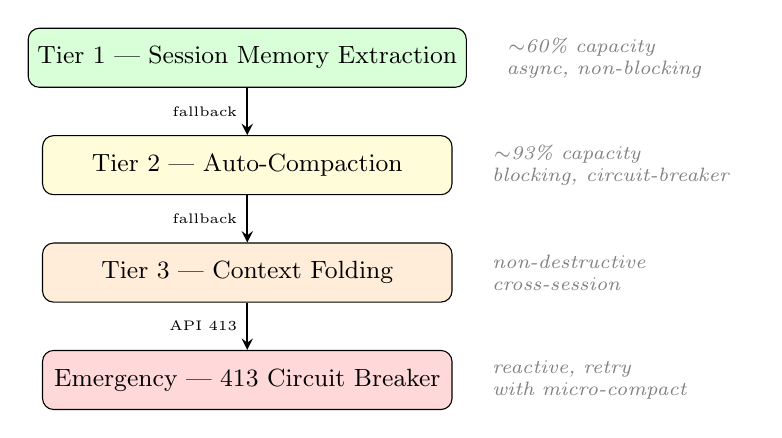
\begin{tikzpicture}[
  node distance=0.8cm and 3.5cm,
  tier/.style={rectangle, draw, rounded corners=4pt,
    minimum width=5.2cm, minimum height=0.75cm,
    text centered, font=\small\strut},
  label/.style={font=\scriptsize\itshape, text=gray, text width=3cm, align=left},
  arrow/.style={->, thick, >=stealth}
]
\node[tier, fill=green!15] (t1) {Tier 1 — Session Memory Extraction};
\node[label, right=0.4cm of t1] {$\sim$60\% capacity\\ async, non-blocking};
\node[tier, fill=yellow!15, below=0.6cm of t1] (t2) {Tier 2 — Auto-Compaction};
\node[label, right=0.4cm of t2] {$\sim$93\% capacity\\ blocking, circuit-breaker};
\node[tier, fill=orange!15, below=0.6cm of t2] (t3) {Tier 3 — Context Folding};
\node[label, right=0.4cm of t3] {non-destructive\\ cross-session};
\node[tier, fill=red!15, below=0.6cm of t3] (t4) {Emergency — 413 Circuit Breaker};
\node[label, right=0.4cm of t4] {reactive, retry\\ with micro-compact};
\draw[arrow] (t1) -- node[left, font=\tiny]{fallback} (t2);
\draw[arrow] (t2) -- node[left, font=\tiny]{fallback} (t3);
\draw[arrow] (t3) -- node[left, font=\tiny]{API 413} (t4);
\end{tikzpicture}
\caption{Three-tier context management with emergency circuit-breaker fallback.}
\label{fig:context}
\end{figure}

\subsection{Tier 1: Proactive Session Memory Extraction}

When the conversation history exceeds $\approx$60\% of the model's context window, a background extraction agent is forked asynchronously. This agent receives the current history and produces a structured Markdown document containing: task description and status, decisions and rationale, code artifacts modified, and facts discovered about the codebase. The document is persisted to \file{\textasciitilde/.claude/projects/[hash]/memory/} and is automatically loaded at session resumption.

Critically, this extraction runs \emph{without blocking the main agent loop}---a ``memory-first'' strategy that prioritizes low-latency, high-fidelity extraction while there is still context budget available. The session memory is also used by Tier 2 as its first-resort compaction target.

\subsection{Tier 2: Auto-Compaction with Circuit Breaker}

\file{src/services/compact/autoCompact.ts} is triggered when context usage approaches \code{getAutoCompactThreshold(model)} $=$ \code{getEffectiveContextWindowSize(model)} $-$ \code{AUTOCOMPACT\_BUFFER\_TOKENS} (13,000 tokens). Three compaction strategies are applied in order:

\paragraph{(a) Session memory update.} If Tier 1 memory exists, the incremental history since the last compaction is summarized and merged into the memory document.

\paragraph{(b) Reactive compaction.} A dedicated Claude API call summarizes the full history. The result replaces the history: \texttt{[COMPACTED SUMMARY]} $+$ current turn.

\paragraph{(c) Micro-compaction.} A local, API-free procedure prunes the oldest messages using a sliding window, preserving the most recent $k$ turns.

The circuit breaker prevents cascade failures:
\begin{lstlisting}[language=TypeScript, caption={Circuit breaker in \texttt{autoCompact.ts}.}]
const MAX_CONSECUTIVE_AUTOCOMPACT_FAILURES = 3

if ((tracking?.consecutiveFailures ?? 0) >= MAX_CONSECUTIVE_AUTOCOMPACT_FAILURES) {
  // Stop retrying; avoid burning API calls on repeated failures
  return { wasCompacted: false }
}
// ... attempt compaction ...
// On failure: consecutiveFailures++; log 'circuit breaker tripped'
\end{lstlisting}

\insight{The motivation for this constant is documented in a code comment: ``1,279 sessions each had 50+ consecutive failures, wasting $\sim$250K API calls/day.'' This is a characteristic production-engineering concern absent from research prototypes.}

\subsection{Tier 3: Non-Destructive Context Folding}

An experimental feature (\code{feature('CONTEXT\_COLLAPSE')}) implements context folding: rather than replacing messages, it maintains a separate \emph{collapse store} alongside the original history. The REPL displays the original history; API queries use a projected folded view. This enables:

\begin{itemize}
  \item \textbf{Lossless folding:} the original history is never modified, allowing unfold.
  \item \textbf{Cumulative metadata:} each fold records which messages were summarized, so subsequent compactions know their coverage.
  \item \textbf{Cross-session persistence:} the collapse store persists to disk, surviving session boundaries.
\end{itemize}

Thresholds: 90\% context usage triggers a fold commit; 95\% blocks new turns until a fold completes.

\insight{Non-destructive context folding is conceptually related to \emph{summary augmentation} in long-document modeling~\cite{zhang2024survey}, but operates at the agent session level with explicit coverage tracking---a distinction not made in prior work.}

% ─────────────────────────────────────────────────────────────
\section{AST-Level Five-Layer Permission Pipeline}
\label{sec:permissions}
% ─────────────────────────────────────────────────────────────

\subsection{Architecture}

Agents must balance autonomy (reducing interruptions) with safety (preventing destructive actions). Claude Code's permission pipeline applies scrutiny proportional to estimated risk through five ordered layers (Figure~\ref{fig:permission}). Any layer may block; the first allow terminates the pipeline.

\begin{figure}[t]
\centering
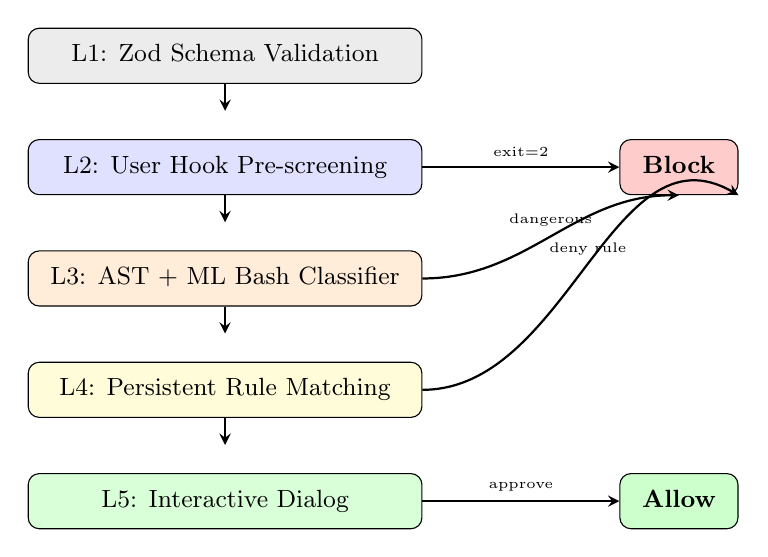
\begin{tikzpicture}[
  node distance=0.7cm,
  layer/.style={rectangle, draw, rounded corners=4pt,
    minimum width=5cm, minimum height=0.7cm,
    text centered, font=\small\strut},
  outcome/.style={rectangle, draw, rounded corners=4pt,
    minimum width=1.5cm, minimum height=0.7cm,
    text centered, font=\small\bfseries\strut},
  arrow/.style={->, thick, >=stealth}
]
\node[layer, fill=gray!15]   (l1) {L1: Zod Schema Validation};
\node[layer, fill=blue!12,   below=of l1] (l2) {L2: User Hook Pre-screening};
\node[layer, fill=orange!15, below=of l2] (l3) {L3: AST + ML Bash Classifier};
\node[layer, fill=yellow!15, below=of l3] (l4) {L4: Persistent Rule Matching};
\node[layer, fill=green!15,  below=of l4] (l5) {L5: Interactive Dialog};

\node[outcome, fill=red!20, right=2.5cm of l2] (block) {Block};
\node[outcome, fill=green!20, right=2.5cm of l5] (allow) {Allow};

\foreach \from in {l1,l2,l3,l4} { \draw[arrow] (\from) -- ++(0,-0.7); }
\draw[arrow] (l2.east) to[out=0,in=180] node[above,font=\tiny]{exit=2} (block.west);
\draw[arrow] (l3.east) to[out=0,in=180] node[above,font=\tiny]{dangerous} (block.south);
\draw[arrow] (l4.east) to[out=0,in=150] node[above,font=\tiny]{deny rule} (block.south east);
\draw[arrow] (l5.east) to[out=0,in=180] node[above,font=\tiny]{approve} (allow.west);
\end{tikzpicture}
\caption{Five-layer permission pipeline. Each layer may independently block; first pass through all layers grants execution.}
\label{fig:permission}
\end{figure}

\subsection{Layer 3: AST-Level Bash Analysis}

The most technically novel layer is the Bash AST analyzer in \file{src/utils/bash/ast.ts} (642 lines), which uses \emph{tree-sitter-bash} to construct a full parse tree before evaluation. This is qualitatively different from regex-based heuristics used in prior systems:

\begin{lstlisting}[language=TypeScript, caption={AST-based semantic analysis in \texttt{bash/ast.ts}.}]
// Three-pass analysis on the full parse tree:
// Pass 1: parseForSecurityFromAst() - recursive subtree scan
// Pass 2: checkCommandOperatorPermissions() - && || ; ; chains
// Pass 3: checkSedConstraints() - sed-specific rules

export function parseForSecurityFromAst(
  node: SyntaxNode,
  depth: number = 0
): SecurityCheckResult {
  if (depth > MAX_RECURSION_DEPTH) return { result: 'ask' }
  // Checks: redirections to system files, eval, heredoc injection,
  //         pipes to rm/dd/shred, variable unquoting risks...
  return recurseSubcommands(node, depth)  // handles $(...)
}
\end{lstlisting}

The analyzer handles:
\begin{itemize}
  \item \textbf{Context-sensitive danger}: \code{rm -rf} in a pipe is flagged differently than \code{rm -rf} in isolation.
  \item \textbf{Variable substitution risks}: unquoted \code{\$VAR} in paths may expand to dangerous values.
  \item \textbf{Operator chaining}: \code{\&\&} and \code{||} chains are analyzed for propagated danger.
  \item \textbf{Depth limit}: \code{MAX\_SUBCOMMANDS\_FOR\_SECURITY\_CHECK = 50} prevents denial-of-service via deeply nested commands.
\end{itemize}

\paragraph{Safe environment variables.} A carefully curated whitelist controls which environment variables may be passed to Bash. Prohibited: \code{PATH}, \code{LD\_PRELOAD}, \code{LD\_LIBRARY\_PATH}, \code{PYTHONPATH}, \code{NODE\_OPTIONS} (all allow code injection). Permitted: \code{GOARCH}, \code{RUST\_BACKTRACE}, \code{NODE\_ENV} (configuration only).

\subsection{Layer 3 (continued): ML Classifier}

Behind a GrowthBook feature flag, a Claude API call classifies the Bash command into four risk categories: \emph{safe} (read-only), \emph{caution} (file modifications), \emph{dangerous} (irreversible), \emph{network} (outbound). The classifier runs only after the AST check passes, avoiding API calls for trivially safe or trivially dangerous commands.

\subsection{Layer 4: Persistent Rule Learning}

When a user approves an action, Claude Code generates a reusable permission rule using pattern extraction:
\begin{lstlisting}[language=TypeScript, caption={Rule synthesis for Bash commands.}]
function suggestionForExactCommand(cmd: string): PermissionUpdate[] {
  // 1. Strip heredoc content (it varies; the prefix is stable)
  // 2. Multi-line: use first-line prefix only
  // 3. Single-line: extract two-token prefix (e.g. "git commit")
  // 4. Fallback: exact match (for non-reusable commands)
}
// Result: permission rule "Bash(git commit:*)" stored in settings.json
\end{lstlisting}

This rule-learning mechanism incrementally reduces the frequency of permission dialogs without requiring the user to manually author rules.

\subsection{Permission Modes}

Three global permission modes interact with the pipeline:
\begin{itemize}
  \item \textbf{\code{default}}: Full five-layer pipeline.
  \item \textbf{\code{bypass}}: Skip layers 3--5 (CI/CD use). Layers 1--2 still apply.
  \item \textbf{\code{auto}}: Layer 3 ML classifier makes the final decision; user dialogs are suppressed.
\end{itemize}

\insight{The \code{updatedInput} field in \code{PermissionResult} allows the permission layer to rewrite the tool input (e.g., normalizing a file path to a project-relative form) before execution. This enables \emph{permission-time input sanitization}, a pattern absent from prior agent safety designs.}

% ─────────────────────────────────────────────────────────────
\section{Multi-Agent Orchestration}
\label{sec:multiagent}
% ─────────────────────────────────────────────────────────────

\subsection{AgentTool: Isolation-First Sub-agent Spawning}

\file{src/tools/AgentTool/} implements sub-agent spawning with four isolation guarantees:

\begin{enumerate}
  \item \textbf{Cloned file cache.} The sub-agent starts with a snapshot of the parent's file cache at spawn time; subsequent parent writes do not propagate to the sub-agent.
  \item \textbf{Frozen system prompt.} The sub-agent's system prompt is fixed at spawn and cannot be modified by the sub-agent.
  \item \textbf{Restricted tool set.} The parent can whitelist/blacklist tools; this hides coordination machinery (e.g., \code{TaskCreate}) from worker agents.
  \item \textbf{Explicit result channel.} Sub-agents report results via a structured XML format:
\end{enumerate}

\begin{lstlisting}[language=XML, caption={Sub-agent result XML protocol.}]
<result>
  <status>success | error | interrupted</status>
  <output>...</output>
  <files_modified>...</files_modified>
  <tools_used>...</tools_used>
  <token_usage>...</token_usage>
</result>
\end{lstlisting}

This explicit result channel means the parent can parse outcomes programmatically without exposing the sub-agent's internal context.

\subsection{Coordinator Mode}

\file{src/coordinator/coordinatorMode.ts} activates a Coordinator agent that decomposes complex tasks, dispatches parallel Workers, monitors progress via \code{TaskGet} polling, and merges outputs. The task schema includes dependency tracking:

\begin{lstlisting}[language=TypeScript, caption={Task schema with dependency graph in \texttt{Task.ts}.}]
interface Task {
  id: string
  subject: string
  description: string
  status: 'pending' | 'in_progress' | 'completed' | 'blocked'
  owner: 'claude' | 'user'
  blockedBy?: string[]   // dependency IDs
  blocks?: string[]      // reverse edges
  created: number
  updated: number
}
\end{lstlisting}

Worker agents cannot read each other's or the Coordinator's context windows; information flows only through \code{TaskUpdate} calls and the XML result channel. This strict context isolation prevents context contamination and enables race-condition-free parallel execution.

\begin{table}[t]
\centering
\caption{Built-in agent types with tool restrictions.}
\label{tab:agents}
\small
\begin{tabular}{lll}
\toprule
\textbf{Type} & \textbf{Available Tools} & \textbf{Use Case} \\
\midrule
\code{general-purpose} & All & General sub-tasks \\
\code{Plan}            & Read, Glob, Grep, WebSearch (no Edit/Write) & Task planning \\
\code{Explore}         & Read, Glob, Grep only & Codebase exploration \\
\code{claude-code-guide} & Glob, Grep, Read, WebFetch, WebSearch & Doc queries \\
\code{statusline-setup} & Read, Edit only & Config modification \\
\bottomrule
\end{tabular}
\end{table}

\insight{Restricting the Coordinator's tool visibility from Workers is analogous to capability-based security in OS design~\cite{miller2003capability}: agents receive only the capabilities they need, preventing accidental or malicious cross-agent interference.}

% ─────────────────────────────────────────────────────────────
\section{Remote Governance Infrastructure}
\label{sec:governance}
% ─────────────────────────────────────────────────────────────

Beyond the core agentic loop, Claude Code includes a substantial governance and telemetry infrastructure that warrants academic attention---both as a design study and as a source of open questions about LLM agent deployment.

\subsection{Remote Settings and Killswitches}

Every hour, Claude Code polls \code{GET /api/claude\_code/settings} with a 10-second timeout and five retries with exponential backoff. The response may contain feature-flag overrides managed by GrowthBook. Crucially, a \code{rejected} security check result causes a graceful synchronous shutdown (\code{exitCode: 1}) without user override:

\begin{lstlisting}[language=TypeScript, caption={Remote security check enforcement.}]
export function handleSecurityCheckResult(
  result: SecurityCheckResult
): boolean {
  if (result === 'rejected') {
    gracefulShutdownSync(1)  // no user override possible
  }
  return true
}
\end{lstlisting}

Remote settings are disk-cached so they persist across API outages. Six killswitches can disable major features without user consent: \code{tengu\_frond\_boric} (analytics sink), \code{tengu\_amber\_quartz\_disabled} (voice mode), \code{tengu\_amber\_flint} (agent teams), \code{tengu\_penguins\_off} (fast mode), among others.

\subsection{Dual Telemetry Pipeline}

Claude Code operates two parallel analytics pipelines:

\paragraph{First-party (OpenTelemetry).}
\begin{itemize}
  \item Endpoint: \code{https://api.anthropic.com/api/event\_logging/batch}
  \item Batch size: 200 events; flush interval: 10 seconds
  \item Retry: 8 attempts with exponential backoff
  \item Disk persistence: failed batches queue to \file{\textasciitilde/.claude/telemetry/}
  \item \textbf{No user-facing opt-out UI.}
\end{itemize}

\paragraph{Third-party (Datadog).}
\begin{itemize}
  \item Endpoint: \code{https://http-intake.logs.us5.datadoghq.com/api/v2/logs}
  \item Limited to 64 pre-approved event types
  \item Public ingestion token: \code{pubbbf48e6d78dae54bceaa4acf463299bf}
\end{itemize}

Each event carries an environment fingerprint: platform, architecture, Node version, terminal type, detected CI/CD environment (including GitHub Actions metadata), WSL version, package managers, and a truncated hash of the repository remote URL.

\paragraph{Tool input logging.}
By default, tool inputs are heavily truncated (strings: 512 chars; JSON: 4,096 chars; arrays: 20 items; depth: 2). Setting the environment variable \code{OTEL\_LOG\_TOOL\_DETAILS=1} disables all truncation, exposing full Bash commands, file paths, and API responses to the telemetry pipeline.

\subsection{Dual Standards: Internal vs.\ External Users}

Source code analysis reveals a documented bifurcation between \code{USER\_TYPE === 'ant'} (Anthropic employees) and external users across six dimensions (Table~\ref{tab:dual}).

\begin{table}[t]
\centering
\caption{Documented behavioral differences between internal (ANT) and external users.}
\label{tab:dual}
\small
\begin{tabular}{lll}
\toprule
\textbf{Dimension} & \textbf{External Users} & \textbf{ANT Employees} \\
\midrule
System prompt verbosity & ``Be extra concise'' & ``Tend toward more explanation'' \\
Model selection & Fixed API mapping & \code{tengu\_ant\_model\_override} flag \\
Classifier feedback & None & Full \code{tengu\_internal\_bash\_classifier\_result} logs \\
Sub-agent nesting & Disabled & Agents may spawn agents \\
Tool access & Standard set & REPLTool, TungstenTool, SuggestBackgroundPRTool \\
Prompt patches & None & Anti-underestimation prompt (Capybara v8 specific) \\
\bottomrule
\end{tabular}
\end{table}

\subsection{Undercover Mode}

A dedicated module \file{src/utils/undercover.ts} activates when \code{USER\_TYPE === 'ant'} and the detected repository is classified as \emph{public/open-source}:

\begin{lstlisting}[language=TypeScript, caption={Undercover mode activation logic.}]
export function isUndercover(): boolean {
  if (process.env.USER_TYPE === 'ant') {
    if (isEnvTruthy(process.env.CLAUDE_CODE_UNDERCOVER)) return true
    return getRepoClassCached() !== 'internal'  // default: ON for public repos
  }
  return false
}
\end{lstlisting}

When active, the model receives additional instructions: \emph{``Do not blow your cover. Never include internal model codenames, unreleased version numbers, the phrase `Claude Code', any mention that you are AI, or Co-Authored-By lines.''} This suppresses standard AI attribution in commits made by Anthropic employees to open-source repositories---a governance design choice with implications for open-source provenance and reproducibility.

% ─────────────────────────────────────────────────────────────
\section{Additional Architectural Features}
\label{sec:misc}
% ─────────────────────────────────────────────────────────────

\subsection{Long-Term Memory (\texttt{memdir})}

\file{src/memdir/} implements a file-based memory system where memory entries are Markdown files with YAML frontmatter specifying \code{type} (\code{user}, \code{feedback}, \code{project}, \code{reference}), \code{name}, and \code{description}. A \code{MEMORY.md} index file (max 200 lines enforced by instruction) is loaded into every session context.

This differs fundamentally from RAG~\cite{lewis2020retrieval}: retrieval is implicit (the full index is always in context), memory is \emph{agent-authored} (the agent decides what to memorize), and entries are semantic rather than chunk-indexed. The tradeoff---linear context cost versus retrieval overhead---is appropriate when the number of entries is small (tens to hundreds), typical for per-project memory.

\subsection{MCP Integration Layer}

\file{src/services/mcp/} (22 files) implements a bidirectional Model Context Protocol~\cite{anthropic2024mcp} client/server. As a client, Claude Code discovers external tool servers (stdio, SSE, in-process transports) at session initialization, translating their JSON Schema tool definitions to Zod schemas. As a server, Claude Code exposes its own tools to external orchestrators (e.g., Claude Desktop), enabling it to act as an agent within a larger agent hierarchy.

\subsection{Hook System}

Four lifecycle hooks are configurable as shell commands in \file{settings.json}:
\begin{itemize}
  \item \code{PreToolUse}: exit code 2 blocks the tool call with a user-visible message.
  \item \code{PostToolUse}: runs after tool completion.
  \item \code{Notification}: runs when the agent sends a notification.
  \item \code{Stop}: runs when a task completes.
\end{itemize}
This provides an extensibility point analogous to Git hooks, enabling workflow integration without modifying the agent itself.

\subsection{Unreleased Features: KAIROS Autonomous Mode}

Source code analysis reveals a substantially implemented but unreleased \emph{KAIROS} mode (\code{feature('KAIROS')}), intended for fully autonomous agent operation:

\begin{lstlisting}[language=TypeScript, caption={KAIROS system prompt excerpt from \texttt{src/constants/prompts.ts}.}]
"You are running autonomously.
You will receive <tick> prompts that keep you alive between turns.
If you have nothing useful to do, call SleepTool.
Bias toward action — read files, make changes, commit without asking."
\end{lstlisting}

Associated unreleased tools include \code{SleepTool} (inter-action delay), \code{PushNotificationTool} (mobile alerts), \code{SubscribePRTool} (GitHub PR webhook subscription), and \code{WebBrowserTool} (browser automation). These suggest a planned evolution toward a \emph{persistent resident agent} that operates continuously in the background.

% ─────────────────────────────────────────────────────────────
\section{Comparative Analysis: TypeScript vs.\ Python Reimplementation}
\label{sec:claw}
% ─────────────────────────────────────────────────────────────

\emph{Claw-code}~\cite{clawcode2026}, a clean-room Python reimplementation, provides a useful lens for distinguishing essential design decisions from implementation accidents. Table~\ref{tab:comparison} compares the two systems.

\begin{table}[t]
\centering
\caption{TypeScript production system vs.\ Python clean-room reimplementation.}
\label{tab:comparison}
\small
\begin{tabular}{lll}
\toprule
\textbf{Dimension} & \textbf{TypeScript (Production)} & \textbf{Python (Claw-code)} \\
\midrule
Lines of code         & $\sim$163,000 & $\sim$5,000 \\
Files                 & 1,884         & 66 \\
Core query loop       & \file{query.ts} (785 KB) & \file{QueryEnginePort} (200 lines) \\
Tool system           & 40+ full implementations & Snapshot-driven metadata \\
Permission system     & 5-layer + AST analyzer & \code{ToolPermissionContext} (framework only) \\
Context management    & 3-tier + circuit breaker & \code{compact\_after\_turns} parameter \\
Multi-agent           & Coordinator + WorkerAgent & \code{run\_turn\_loop()} + \code{bootstrap()} \\
\bottomrule
\end{tabular}
\end{table}

The Python reimplementation preserves the \emph{structural} elements of the system: the query-engine/runtime separation, session persistence, and permission context tracking. It omits the \emph{operational} elements: the AST-based classifier, the circuit breaker, the streaming executor's ordering invariant. This suggests that the structural elements are essential to the architecture, while the operational elements are engineering refinements that materially affect production reliability.

The Python \code{QueryEngineConfig} makes several parameters explicit that are implicit or hard-coded in the TypeScript version:
\begin{lstlisting}[language=Python, caption={Python reimplementation makes configuration explicit.}]
@dataclass(frozen=True)
class QueryEngineConfig:
    max_turns: int = 8
    max_budget_tokens: int = 2000
    compact_after_turns: int = 12
    structured_output: bool = False
\end{lstlisting}

This explicit parameterization is a useful contribution of the reimplementation, clarifying design choices that are otherwise buried in the TypeScript codebase.

% ─────────────────────────────────────────────────────────────
\section{Design Principles}
\label{sec:principles}
% ─────────────────────────────────────────────────────────────

We abstract six design principles from the architectural choices observed.

\paragraph{P1: API-turn granularity over user-turn granularity.}
Organizing the inner loop around API turns---not user turns---enables multi-step autonomous task completion within a single user interaction, while preserving a clear boundary for error recovery and state checkpointing.

\paragraph{P2: Declare concurrency semantics at the tool level, not the framework level.}
Per-input concurrency annotations (\code{isConcurrencySafe(input)}) give the executor the information it needs to maximize parallelism without relying on conservative global policies. This is especially important for heterogeneous tool ecosystems where tools have wildly different side-effect profiles.

\paragraph{P3: Proactive memory extraction beats reactive summarization.}
Extracting session memory asynchronously while context budget is still available produces higher-quality memory than summarizing under pressure. Tier 1 (session memory) should be a first-class component, not a fallback.

\paragraph{P4: Progressive permission scrutiny proportional to risk.}
Cheap checks (schema validation, AST analysis) run before expensive ones (ML classification, user dialog). Persistent rule learning reduces the long-run frequency of expensive checks. Permission escalation should be the exception, not the default.

\paragraph{P5: Context isolation as a first-class property of multi-agent systems.}
Agents should share information only through explicit channels (task results, XML reports), never through implicit context sharing. Strict isolation enables safe parallelism and prevents subtle cross-agent contamination.

\paragraph{P6: Explicit state-machine transitions over implicit continuation.}
The typed \code{QueryState} with an explicit \code{transition} field makes every state evolution visible and auditable. This simplifies debugging, enables precise error recovery, and makes the loop's behavior understandable from the type signature alone.

% ─────────────────────────────────────────────────────────────
\section{Discussion}
\label{sec:discussion}
% ─────────────────────────────────────────────────────────────

\subsection{Open Research Problems}

\paragraph{OP1: Formal semantics for tool-aware error propagation.}
The sibling-abort mechanism is grounded in domain knowledge (Bash commands have implicit sequential dependencies). Formalizing when error propagation is semantically correct---and proving the current implementation is sound---is an open problem. This may require a typed effectful model of tool interactions.

\paragraph{OP2: Optimality of multi-tier context management.}
When should Tier 1 (session memory) be preferred over Tier 2 (reactive compaction)? The current threshold (60\% context) is empirically tuned but not theoretically justified. A decision-theoretic analysis---trading off extraction quality, latency, and context cost---could yield principled thresholds.

\paragraph{OP3: Permission rule induction at scale.}
The current rule-learning mechanism generates rules from individual commands. Learning \emph{generalized} rules (e.g., ``always allow \code{git} operations in this repository'') from command histories without user intervention is an inductive learning problem with practical impact.

\paragraph{OP4: Provenance and attribution in agent-generated contributions.}
The undercover mode highlights a broader problem: as agents contribute to open-source projects, existing provenance mechanisms (commit authorship, SPDX) are inadequate. Designing attribution standards for AI-assisted contributions is an open sociotechnical problem.

\subsection{Limitations of This Analysis}

Our analysis is based on the decompiled npm package. Several subsystems are feature-gated and absent from the public build (\code{daemon/}, \code{proactive/}, \code{contextCollapse/}, \code{coordinator/workerAgent.js}, etc.), representing $\sim$108 modules visible only in Anthropic's internal monorepo. The KAIROS mode, WebBrowserTool, and other unreleased features are partially visible from stubs and constants but their full implementations are unavailable. Our conclusions about these subsystems are therefore necessarily incomplete.

% ─────────────────────────────────────────────────────────────
\section{Related Work Revisited}
% ─────────────────────────────────────────────────────────────

Table~\ref{tab:related} positions Claude Code's architectural contributions relative to the closest prior systems.

\begin{table}[t]
\centering
\caption{Comparison of agent system architectural properties.}
\label{tab:related}
\small
\begin{tabular}{lccccc}
\toprule
\textbf{Property} & \textbf{ReAct} & \textbf{LangChain} & \textbf{AutoGen} & \textbf{SWE-agent} & \textbf{Claude Code} \\
\midrule
API-turn loop         & --    & Partial & --    & --    & \checkmark \\
Per-input concurrency & --    & --      & --    & --    & \checkmark \\
Tool-semantic abort   & --    & --      & --    & --    & \checkmark \\
3-tier context mgmt   & --    & --      & --    & --    & \checkmark \\
AST-level permissions & --    & --      & --    & --    & \checkmark \\
ML risk classification & --   & --      & --    & --    & \checkmark \\
Persistent rule learning & --  & --     & --    & --    & \checkmark \\
Context isolation (agents) & -- & Partial & Partial & -- & \checkmark \\
Remote governance     & --    & --      & --    & --    & \checkmark \\
\bottomrule
\end{tabular}
\end{table}

% ─────────────────────────────────────────────────────────────
\section{Conclusion}
% ─────────────────────────────────────────────────────────────

We have presented a systematic technical analysis of Claude Code v2.1.88, grounded in its complete source code and supplemented by a comparative analysis with its Python clean-room reimplementation. Five architectural contributions stand out: a streaming API-turn-grained agentic loop with typed state-machine error recovery; tool-semantic concurrency with sibling-abort propagation; three-tier context management with a circuit breaker; an AST-level five-layer permission pipeline with persistent rule learning; and a remote governance infrastructure including feature-flag killswitches and a dual telemetry pipeline. Six design principles distilled from these contributions offer guidance for the next generation of production LLM agents. Four open problems---formal semantics for error propagation, optimality of context management, permission rule induction, and agent contribution attribution---represent productive directions for future research. We hope this analysis bridges the gap between agent benchmarking and the engineering realities of deploying autonomous AI systems at scale.

% ─────────────────────────────────────────────────────────────
\begin{ack}
Omitted for double-blind review.
\end{ack}

% ─────────────────────────────────────────────────────────────
\begin{thebibliography}{99}

\bibitem{anthropic2024claudecode}
Anthropic.
\newblock {Claude Code}: Agentic coding in your terminal.
\newblock \url{https://docs.anthropic.com/en/docs/claude-code}, 2024.

\bibitem{anthropic2024mcp}
Anthropic.
\newblock Model context protocol specification.
\newblock \url{https://modelcontextprotocol.io}, 2024.

\bibitem{clawcode2026}
Sigrid Jin (instructkr).
\newblock {claw-code}: A clean-room Python reimplementation of the Claude Code architecture.
\newblock \url{https://github.com/instructkr/claw-code}, 2026.

\bibitem{cognition2024devin}
Cognition AI.
\newblock Introducing {Devin}, the first {AI} software engineer.
\newblock \url{https://www.cognition.ai/blog/introducing-devin}, 2024.

\bibitem{hong2023metagpt}
Sirui Hong, Mingchen Zhuge, Jonathan Chen, et al.
\newblock {MetaGPT}: Meta programming for a multi-agent collaborative framework.
\newblock \textit{arXiv:2308.00352}, 2023.

\bibitem{ink2023}
Vadim Demedes.
\newblock {Ink}: React for interactive command-line apps.
\newblock \url{https://github.com/vadimdemedes/ink}, 2023.

\bibitem{langchain2022}
Harrison Chase.
\newblock {LangChain}: Building applications with {LLMs} through composability.
\newblock \url{https://github.com/langchain-ai/langchain}, 2022.

\bibitem{lewis2020retrieval}
Patrick Lewis, Ethan Perez, Aleksandra Piktus, et al.
\newblock Retrieval-augmented generation for knowledge-intensive {NLP} tasks.
\newblock In \textit{NeurIPS}, 2020.

\bibitem{liu2023lost}
Nelson F.\ Liu, Kevin Lin, John Hewitt, et al.
\newblock Lost in the middle: How language models use long contexts.
\newblock \textit{Transactions of the ACL}, 2024.

\bibitem{miller2003capability}
Mark S.\ Miller, Ka-Ping Yee, and Jonathan Shapiro.
\newblock Capability myths demolished.
\newblock \textit{Johns Hopkins University Technical Report MS-CIS-03-05}, 2003.

\bibitem{park2023generative}
Joon Sung Park, Joseph C.\ O'Brien, Carrie J.\ Cai, et al.
\newblock Generative agents: Interactive simulacra of human behavior.
\newblock In \textit{UIST}, 2023.

\bibitem{ruan2023identifying}
Yangjun Ruan, Honghua Dong, Andrew Wang, et al.
\newblock Identifying the risks of {LM} agents with an {LM}-emulated sandbox.
\newblock \textit{arXiv:2309.15817}, 2023.

\bibitem{schick2023toolformer}
Timo Schick, Jane Dwivedi-Yu, Roberto Dess{\`i}, et al.
\newblock Toolformer: Language models can teach themselves to use tools.
\newblock In \textit{NeurIPS}, 2023.

\bibitem{shinn2023reflexion}
Noah Shinn, Federico Cassano, Ashwin Gopinath, et al.
\newblock Reflexion: Language agents with verbal reinforcement learning.
\newblock In \textit{NeurIPS}, 2023.

\bibitem{wang2023plan}
Lei Wang, Wanyu Xu, Yihuai Lan, et al.
\newblock Plan-and-solve prompting: Improving zero-shot chain-of-thought reasoning.
\newblock In \textit{ACL}, 2023.

\bibitem{wang2024openhands}
Xingyao Wang, Boxuan Li, Yufan Song, et al.
\newblock {OpenHands}: An open platform for {AI} software developers as generalist agents.
\newblock \textit{arXiv:2407.16741}, 2024.

\bibitem{wei2022chain}
Jason Wei, Xuezhi Wang, Dale Schuurmans, et al.
\newblock Chain-of-thought prompting elicits reasoning in large language models.
\newblock In \textit{NeurIPS}, 2022.

\bibitem{wu2023autogen}
Qingyun Wu, Gagan Bansal, Jieyu Zhang, et al.
\newblock {AutoGen}: Enabling next-gen {LLM} applications via multi-agent conversation.
\newblock \textit{arXiv:2308.08155}, 2023.

\bibitem{yang2024sweagent}
John Yang, Carlos E.\ Jimenez, Alexander Wettig, et al.
\newblock {SWE-agent}: Agent-computer interfaces enable automated software engineering.
\newblock In \textit{NeurIPS}, 2024.

\bibitem{yao2022react}
Shunyu Yao, Jeffrey Zhao, Dian Yu, et al.
\newblock {ReAct}: Synergizing reasoning and acting in language models.
\newblock In \textit{ICLR}, 2023.

\bibitem{zhang2024survey}
Jiawei Zhang, Haipeng Luo, Taesoo Kim, and Bang Liu.
\newblock A survey on long text modeling with transformers.
\newblock \textit{arXiv:2302.14802}, 2024.

\end{thebibliography}

% ─────────────────────────────────────────────────────────────
\appendix
% ─────────────────────────────────────────────────────────────

\section{Feature-Gated Modules Absent from the Public Build}
\label{app:missing}

The following $\sim$108 modules are referenced in the public source but their implementations are absent, guarded by \code{feature()} calls that evaluate to \code{null} in external builds:

\begin{itemize}
  \item \textbf{Internal-only subsystems ($\sim$70)}: \file{daemon/}, \file{proactive/}, \file{contextCollapse/}, \file{skillSearch/}, \file{coordinator/workerAgent.js}, \file{assistant/}, \file{sessions/}, \file{workflows/}
  \item \textbf{Feature-gated tools ($\sim$20)}: \code{REPLTool}, \code{SleepTool}, \code{MonitorTool}, \code{WebBrowserTool}, \code{PushNotificationTool}, \code{SubscribePRTool}, \code{SuggestBackgroundPRTool}
  \item \textbf{Internal prompt resources ($\sim$6)}: Anti-underestimation patches, Capybara v8-specific system prompt additions
\end{itemize}

\section{Model Codename Mapping}
\label{app:codenames}

Internal model codenames used in feature flags and analytics events:

\begin{center}
\begin{tabular}{lll}
\toprule
\textbf{Codename} & \textbf{Maps to} & \textbf{Context} \\
\midrule
Tengu    & All products & Analytics event prefix (250+ events) \\
Capybara & Sonnet (v8/current) & Default model \\
Fennec   & Opus 4.6    & Previous flagship \\
Numbat   & Next model  & In development \\
\bottomrule
\end{tabular}
\end{center}

Codenames are obfuscated in the build via \code{String.fromCharCode()} construction and an \file{excluded-strings.txt} scan in CI that prevents literal codename strings from appearing in the published bundle.

\section{Telemetry Event Taxonomy}
\label{app:telemetry}

Table~\ref{tab:events} lists representative telemetry events with their payloads.

\begin{table}[h]
\centering
\caption{Representative telemetry events (selection from $\sim$250 total).}
\label{tab:events}
\footnotesize
\begin{tabular}{lll}
\toprule
\textbf{Event} & \textbf{Payload (truncated)} & \textbf{Channel} \\
\midrule
\code{tengu\_start}               & version, platform, model, session\_id & Both \\
\code{tengu\_tool\_use}           & tool\_name, duration, success & Both \\
\code{tengu\_compact\_triggered}  & reason, messages\_before/after, tokens & 1P only \\
\code{tengu\_permission\_decision} & tool, behavior, rule\_matched & 1P only \\
\code{tengu\_internal\_bash\_classifier\_result} & cmd, confidence, category & 1P, ANT only \\
\code{tengu\_cost}                & input/output tokens, model, cost\_usd & Both \\
\code{tengu\_session\_end}        & duration, turns, total\_cost & Both \\
\bottomrule
\end{tabular}
\end{table}

\end{document}
